\chapter{Конструкторский раздел}	
В конструкторской части разработано программное обеспечение, а также формально описаны применяемые алгоритмы.

\section{Схемы алгоритмов визуализации трехмерной сцены}
\subsection{Алгоритм, использующий z-буфер}
На рисунках~\ref{fig:z_buf_2} представлена схема алгоритма с использованием z-буфера.
%\begin{figure}[H]%
%	\centering
%	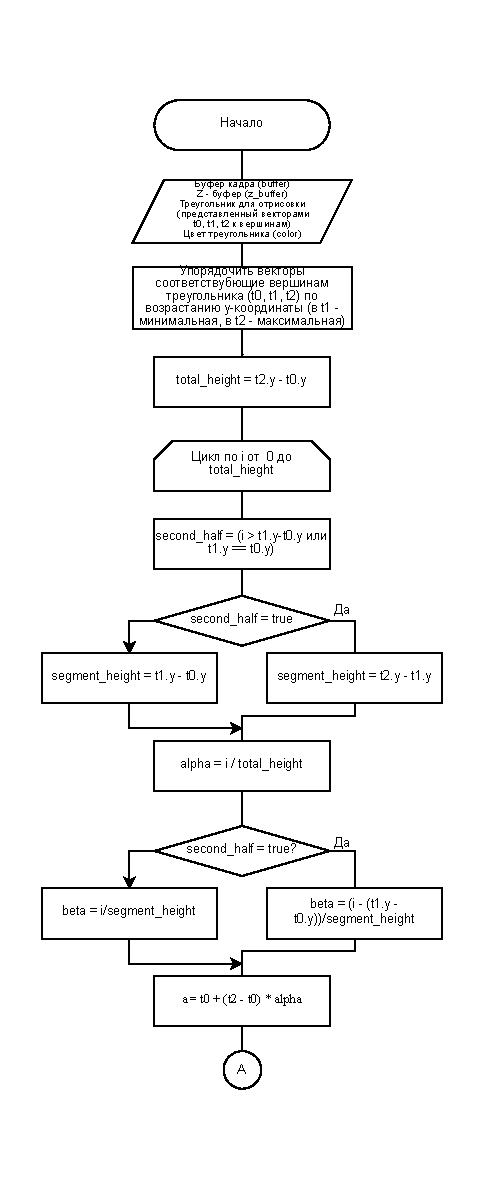
\includegraphics[width=0.6\textwidth, page=1]{assets/img/z-bufer.pdf}   
%	\caption{Схема алгоритма с использованием z-буфера}
%	\label{fig:z_buf_1}
%\end{figure}

%\begin{figure}[H]
%	\centering
%	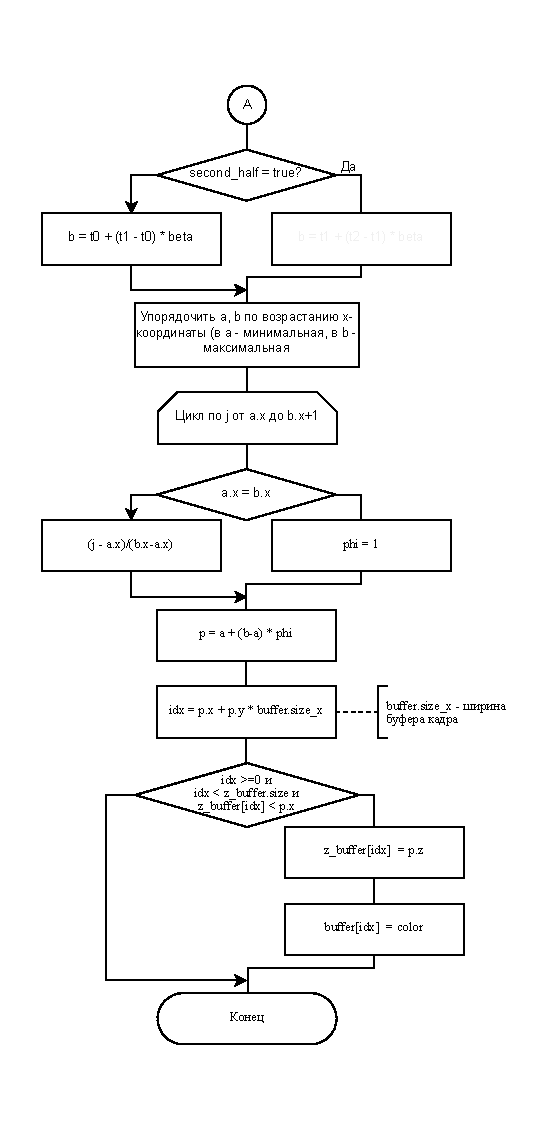
\includegraphics[width=0.6\textwidth, page=1]{assets/img/z-bufer_2.pdf}   
%	\caption{Схема алгоритма с использованием z-буфера}
%	\label{fig:z_buf_2}
%\end{figure}

\begin{figure}[H]
	\centering
	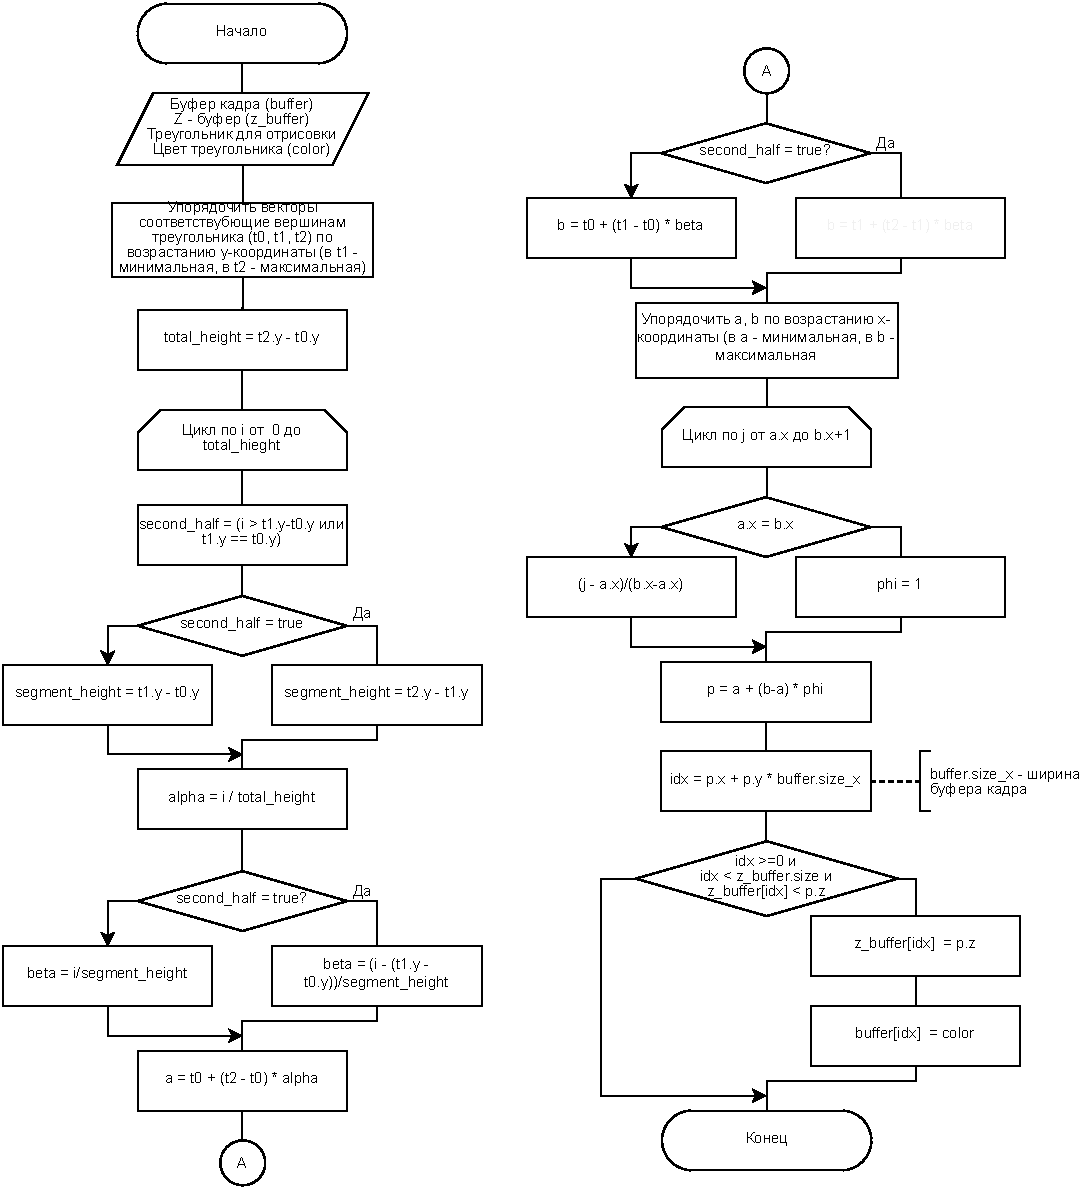
\includegraphics[width=1.0\textwidth, page=1]{assets/img/z-bufer-full.pdf}   
	\caption{Схема алгоритма с использованием z-буфера}
	\label{fig:z_buf_2}
\end{figure}

\subsection{Алгоритм поведения газов}

На рисунке~\ref{fig:Navie-Stocks} представлена схема алгоритма поведения газа на основе уравнений Навье---Стокса. 
\begin{figure}[H]
	\centering
	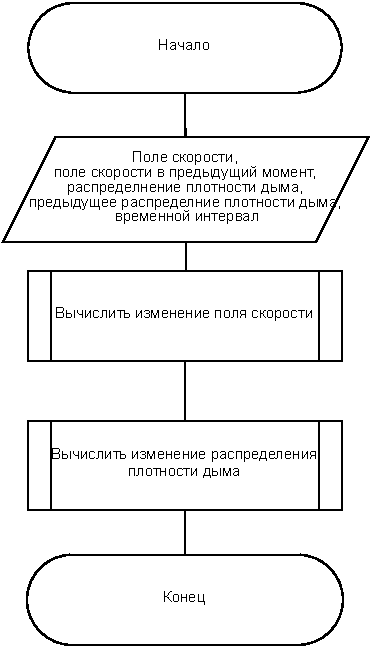
\includegraphics[width=0.7\textwidth, page=1]{assets/img/Naive_stocks.pdf}   
	\caption{Схема алгоритма на основе уравнения Навье---Стокса}
	\label{fig:Navie-Stocks}
\end{figure}

На рисунке~\ref{fig:dens_step} представлена схема алгоритма обновления распределения плотности дыма.

\begin{figure}[H]
	\centering
	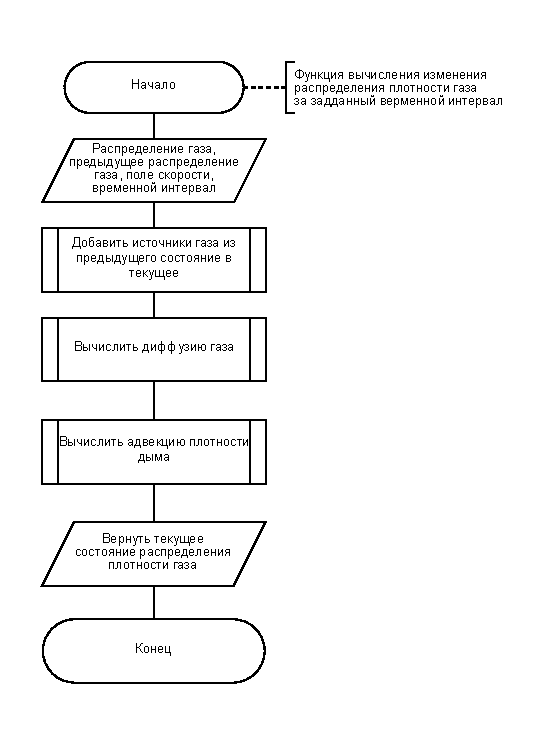
\includegraphics[width=0.8\textwidth, page=1]{assets/img/dens_step.pdf}   
	\caption{Схема алгоритма обновления распределения плотности дыма}
	\label{fig:dens_step}
\end{figure}

На рисунке~\ref{fig:vel_step} представлена схема алгоритма обновления поля скорости.

\begin{figure}[H]
	\centering
	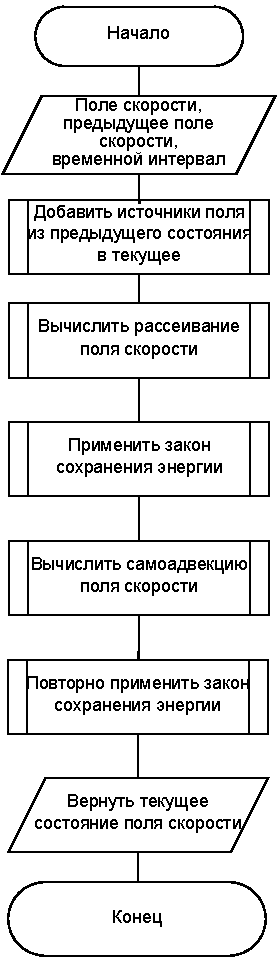
\includegraphics[width=0.8\textwidth, page=1]{assets/img/velocity_step.pdf}   
	\caption{Схема алгоритма обновления распределения плотности газа}
	\label{fig:vel_step}
\end{figure}

На рисунке~\ref{fig:add_src} представлена схема алгоритма добавления источников в систему, используемая как в алгоритме обновления поля скорости, так и в алгоритме обновления распределения плотности дыма.

\begin{figure}[H]
	\centering
	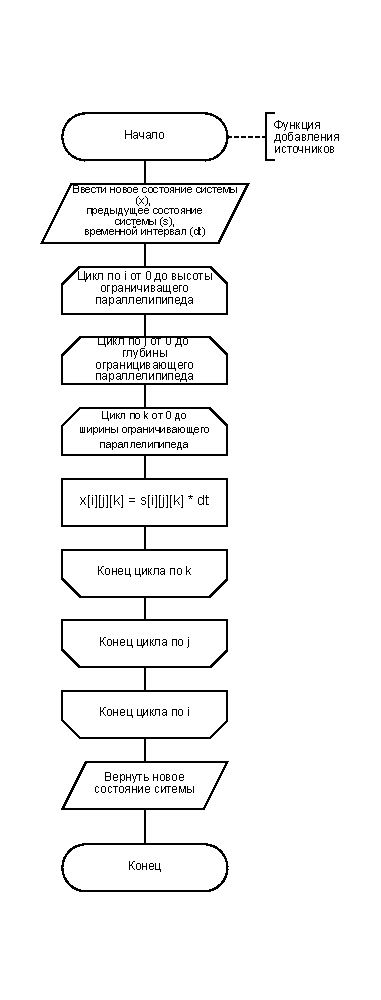
\includegraphics[width=0.5\textwidth, page=1]{assets/img/add_source.pdf}
	\caption{Схема алгоритма добавления источников в систему}
	\label{fig:add_src}
\end{figure}

На рисунке~\ref{fig:lin_solve} представлена схема алгоритма решения СЛАУ, основанного на методе Гаусса---Зейделя.

\begin{figure}[H]
	\centering
	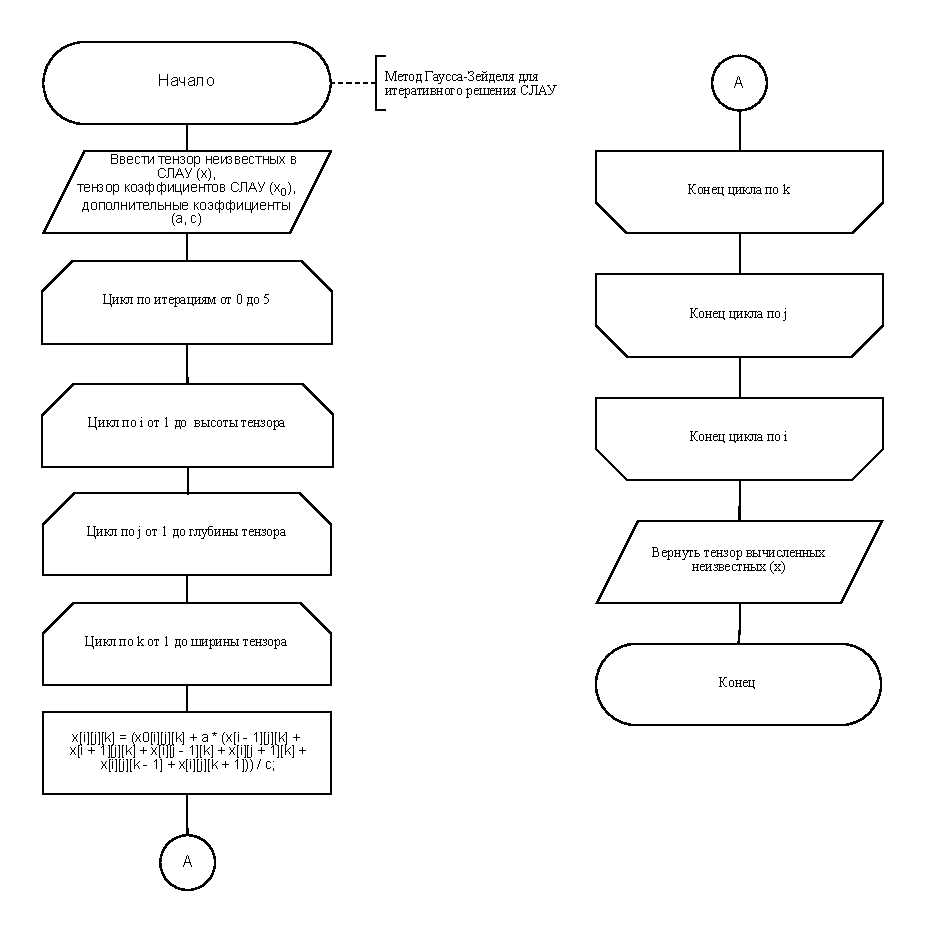
\includegraphics[width=1.0\textwidth,page=1]{assets/img/gauss-zeidel.pdf}
	\caption{Схема алгоритма решения СЛАУ}
	\label{fig:lin_solve}
\end{figure}

В обоих случаях под диффузией предполагается обмен ячейки ограничивающего параллелепипеда плотностью или скоростью с соседними по граням ячейками. Пример для двухмерной симуляции представлен на рисунке~\ref{fig:diffusion}.

\begin{figure}[H]
	\centering
	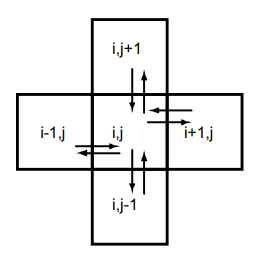
\includegraphics[width=0.4\textwidth, page=1]{assets/img/diffusion.png}   
	\caption{Пример диффузии для двумерной симуляции}
	\label{fig:diffusion}
\end{figure}



На рисунке~\ref{fig:diffuse} представлена схема алгоритма вычисления диффузии (рассеивания), используемого для обновления поля скорости и распределения плотности газа.

\begin{figure}[H]
	\centering
	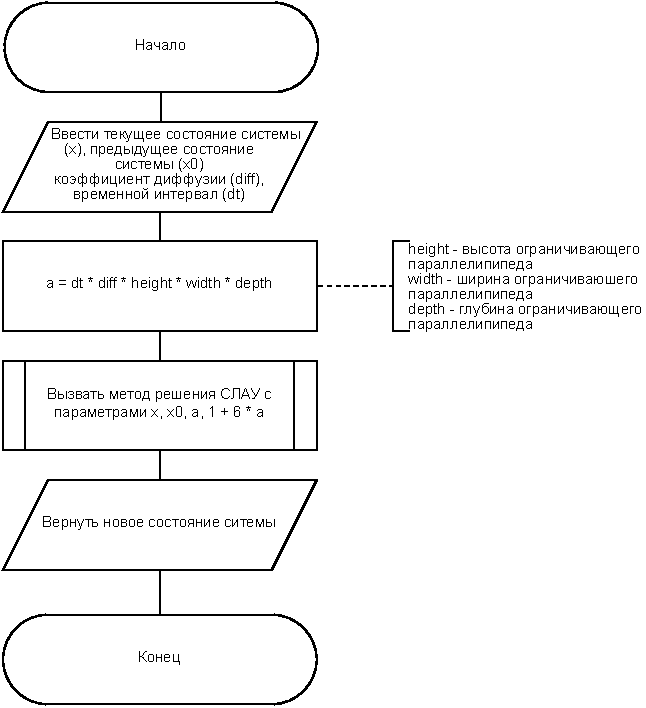
\includegraphics[width=1.0\textwidth,page=1]{assets/img/diffuse.pdf}
	\caption{Схема алгоритма вычисления диффузии (рассеивания)}
	\label{fig:diffuse}
\end{figure}

На рисунке~\ref{fig:advect} представлена схема алгоритма вычисления адвекции и самоадвекции для распределение плотности и поля скорости соответственно.


\begin{figure}[H]
	\centering
	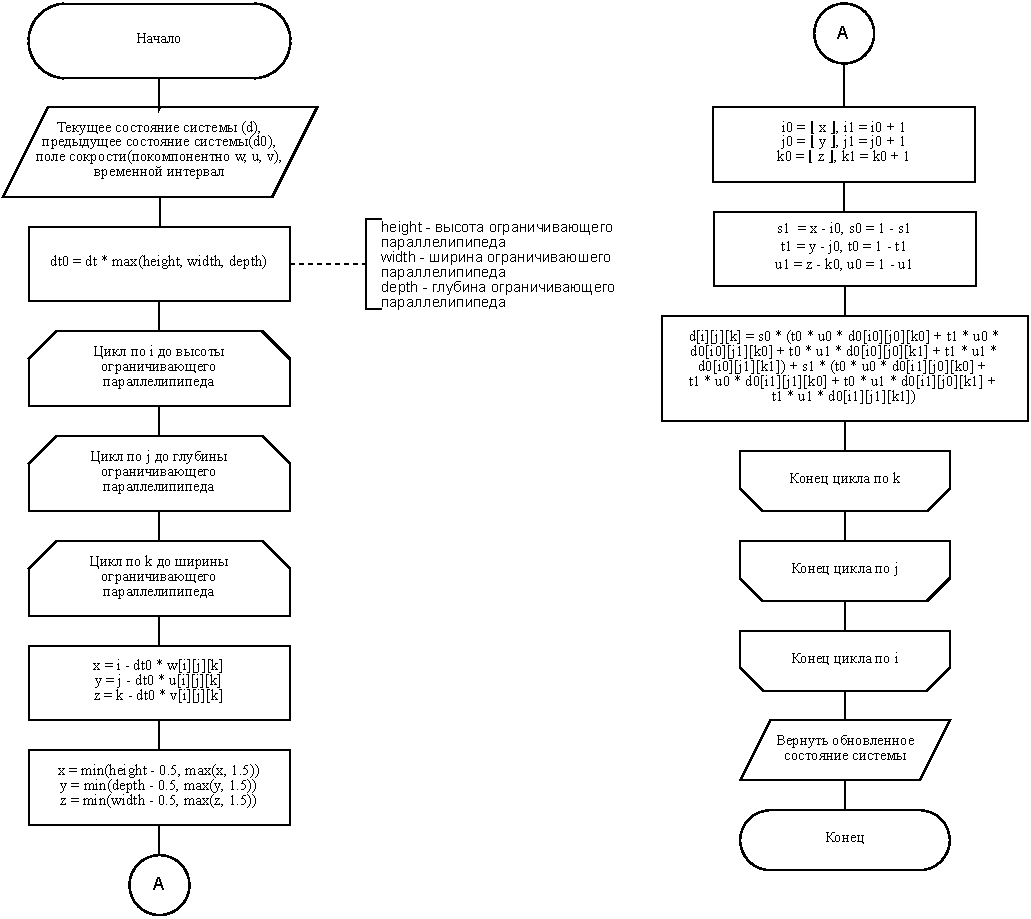
\includegraphics[width=1.0\textwidth,page=1]{assets/img/advect.pdf}
	\caption{Схема алгоритма вычисления адвекции}
	\label{fig:advect}
\end{figure}

\section{Диаграмма классов}

На рисунке~\ref{fig:uml} представлена UML-диаграмма классов программного обеспечения.

\begin{figure}[H]
	\centering
	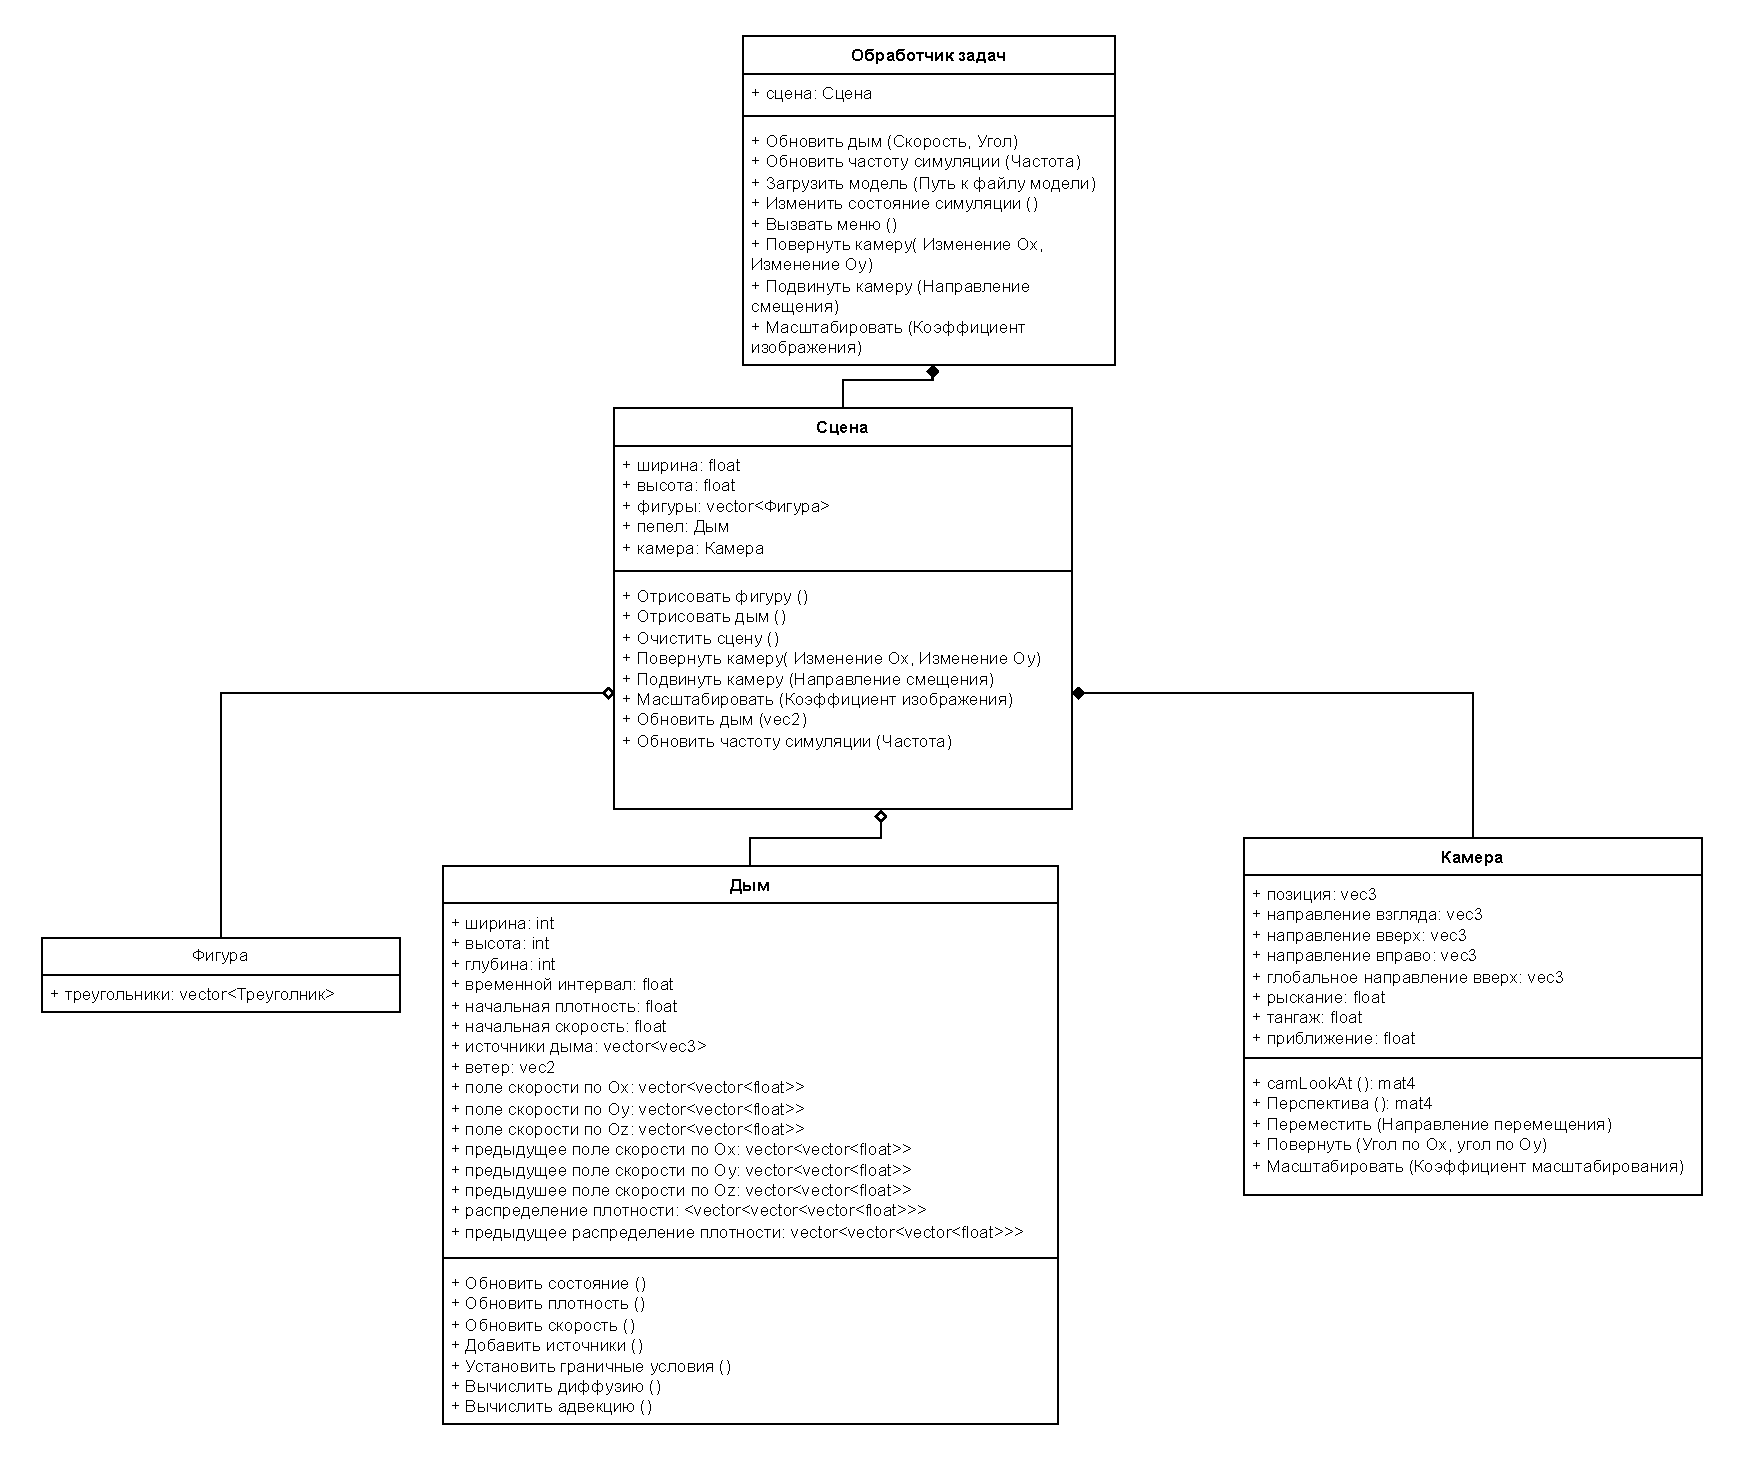
\includegraphics[width=0.9\textwidth,page=1]{assets/img/smoke_uml.pdf}
	\caption{UML-диаграмма классов}
	\label{fig:uml}
\end{figure}

\section*{Вывод}
В разделе спроектировано разрабатываемое программное обеспечение для визуализации извержения вулкана, приведены схемы алгоритмов и UML-диаграмма классов ПО.
